\input{childdoc.def}
\childdocmain{}

%{\def\ignore{\usepackage{ws-procs9x6}}}%disable hyper at arxiv
{\def\ignore{\pdfoutput=1}}%use pdflatex at arxiv

\documentclass[11pt,a4paper,openany]{book}

%%%%%%%%%%%%%%%%%%%%%%%%%%%%%%%%%%%%%%%%%%%%
%%%%%%%%%%%%%%%%%%%%%%%%%%%%%%%%%%%%
%% Page layout 
\usepackage[a4paper,text={160mm,247mm},centering]{geometry}
% setspace does proper distances between lines, but leaves footnotes etc. intact
\usepackage{setspace}
\usepackage{rotating}
\usepackage{mathfixs}
\setstretch{1.1}

%% Fonts and languages
\usepackage[T1]{fontenc}
\usepackage[utf8]{inputenc}
\usepackage[icelandic,english]{babel}

%%%%%%%%%%%%%%%%%%%%%%%%%%%%%%%%%%%%%%%%%%%%
%%%%%%%%%%%%%%%%%%%%%%%%%%%%%%%%%%%%
%% Fancy headers, if desired
%\usepackage{fancyhdr, dsfont}
%\renewcommand{\headrulewidth}{0.4pt}
%\renewcommand{\footrulewidth}{0.4pt}

%%%%%%%%%%%%%%%%%%%%%%%%%%%%%%%%%%%%%%%%%%%%
%%%%%%%%%%%%%%%%%%%%%%%%%%%%%%%%%%%%
% Several Packages: Math, Graphics
\usepackage{amsmath, amssymb, amsfonts, geometry}
\usepackage{amsthm}

\usepackage{mathrsfs}
\usepackage{txfonts}
\usepackage{braket}

% \usepackage{showlabels}

\usepackage{lipsum}
%%%%%%%%%%%%%%%%%%%%%%%%%%%%%%%%%%%%%%%%%%%%%%%%%%%%%%%%%%%%%%%%%%%%%%%%%%%%%%
%%%%%  METAPOST / Colors / Graphics
%%%%%%%%%%%%%%%%%%%%%%%%%%%%%%%%%%%%%%%%%%%%%%%%%%%%%%%%%%%%%%%%%%%%%%%%%%%%%%
\usepackage[compile=false,fonts]{mpostinl}
%\usepackage{graphbox}
%\pdfminorversion=5
%\pdfcompresslevel=9
%\pdfobjcompresslevel=3

%%%%%%%%%%%%%%%%%%%%%%%%%%%%%%%%%%%%%%%%%%%%%%%%%%%%%%%%%%%%%%%%%%%%%%%%%%%%%%
%%%%%  Define some nice colors
%%%%%%%%%%%%%%%%%%%%%%%%%%%%%%%%%%%%%%%%%%%%%%%%%%%%%%%%%%%%%%%%%%%%%%%%%%%%%%
%\usepackage{xcolor}
\usepackage[usenames,dvipsnames,table]{xcolor}
\definecolor{mygreen}{rgb}{0,0.4,0}
\definecolor{myblue}{rgb}{0,0.0,0.4}
\definecolor{refrcolor}{rgb}{0,0.4,0}
\definecolor{cgreen}{rgb}{0,0.7,0}
\definecolor{ecolor}{rgb}{.52,.03,.06}
\definecolor{bgcolor}{rgb}{.96,.95,.80}
\definecolor{bgcolordark}{rgb}{.80,.80,.67}
\definecolor{faint}{rgb}{.80,.80,.80}
\definecolor{myred}{rgb}{0.55,0.0,0.05}

%%%%%%%%%%%%%%%%%%%%%%%%%%%%%%%%%%%%%%%%%%%%%%%%%%%%%%%%%%%%%%%%%%%%%%%%%%%%%%
%%%%%  Define some nice colors
%%%%%%%%%%%%%%%%%%%%%%%%%%%%%%%%%%%%%%%%%%%%%%%%%%%%%%%%%%%%%%%%%%%%%%%%%%%%%%

%%%%%%%%%%%%%%%%%%%%%%%%%%%%%%%%%%%%%%%%%%%%%%%%%%%%%%%%%%%%%%%%%%%%%%%%%%%%%%
%%%%%  Enumitem
%%%%%%%%%%%%%%%%%%%%%%%%%%%%%%%%%%%%%%%%%%%%%%%%%%%%%%%%%%%%%%%%%%%%%%%%%%%%%%
\usepackage{enumitem}

%%%%%%%%%%%%%%%%%%%%%%%%%%%%%%%%%%%%%%%%%%%%%%%%%%%%%%%%%%%%%%%%%%%%%%%%%%%%%%
%%%%%  Hacks for particular reports.
%%%%%%%%%%%%%%%%%%%%%%%%%%%%%%%%%%%%%%%%%%%%%%%%%%%%%%%%%%%%%%%%%%%%%%%%%%%%%%

%added for report A1 to work
\usepackage[framemethod=default]{mdframed}
\newmdtheoremenv[backgroundcolor=black!10,linewidth=0pt]{definition}{Definition}[chapter]
\newmdtheoremenv[backgroundcolor=black!10,linewidth=0pt]{theorem}{Theorem}[chapter]
\newmdtheoremenv[backgroundcolor=black!10,linewidth=0pt]{lemma}{Lemma}[chapter]
%\newtheorem{definition}{Definition}
%\newtheorem{theorem}{Theorem}
%added for report A3 to work
\DeclareMathOperator{\I}{I}

%added for report B2 to work
\usepackage{wrapfig}
%added for report B3 to work
\usepackage{amsthm}
%added for report B3 to work
\usepackage{relsize}
%added for report D2 to work
\usepackage{mathtools}
\usepackage{listings}

%added for report E3 to work
%\usepackage{standalone}
%%%%%%%%%%%%%%%%%%%%%%%%%%%%%%%%%%%%%%%%%%%%%%%%%%%%%%%%%%%%%%%%%%%%%%%%%%%%%%
%%%%%  Include the METAPOST drawing setup
%%%%%%%%%%%%%%%%%%%%%%%%%%%%%%%%%%%%%%%%%%%%%%%%%%%%%%%%%%%%%%%%%%%%%%%%%%%%%%

%\input{drinfeldmp}

%%%%%%%%%%%%%%%%%%%%%%%%%%%%%%%%%%%%%%%%%%%%
%%%%%%%%%%%%%%%%%%%%%%%%%%%%%%%%%%%%
% The package "shuffle" is using old pi-type fonts which are not 
% properly treated in several modern text-processing systems. In 
% particular publishing with IOP (JPhysA) causes serious trouble. 
% The following tex-code provides a reasonable shuffle symbol. 
% \usepackage{shuffle}

\makeatletter
\providecommand*{\shuffle}{%
  \mathbin{\mathpalette\shuffle@{}}%
}
\newcommand*{\shuffle@}[2]{%
  % #1: math style
  % #2: unused
  \sbox0{$#1\vcenter{}$}%
  \kern .15\ht0 % side bearing
  \rlap{\vrule height .25\ht0 depth 0pt width 2.5\ht0}%
  \raise.1\ht0\hbox to 2.5\ht0{%
    \vrule height 1.75\ht0 depth -.1\ht0 width .17\ht0 %
    \hfill
    \vrule height 1.75\ht0 depth -.1\ht0 width .17\ht0 %
    \hfill
    \vrule height 1.75\ht0 depth -.1\ht0 width .17\ht0 %
  }%
  \kern .15\ht0 % side bearing
}
\makeatother

%%%%%%%%%%%%%%%%%%%%%%%%%%%%%%%%%%%%%%%%%%%%
%%%%%%%%%%%%%%%%%%%%%%%%%%%%%%%%%%%%
% automatic bold math in headlines
\makeatletter
\g@addto@macro\bfseries{\boldmath}
\makeatother

%%%%%%%%%%%%%%%%%%%%%%%%%%%%%%%%%%%%%%%%%%%%
%%%%%%%%%%%%%%%%%%%%%%%%%%%%%%%%%%%%
% change appearance of the table of contents
\usepackage{tocloft}
\setlength{\cftchapnumwidth}{2.4em}
\setlength{\cftsecindent}{2.5em}
\setlength{\cftsecnumwidth}{1.8em}
\setlength{\cftsubsecindent}{4.3em}
\setlength{\cftsubsecnumwidth}{2.7em}

\addto\captionsenglish{\renewcommand{\chaptername}{Report}}

%%%%%%%%%%%%%%%%%%%%%%%%%%%%%%%%%%%%%
%%%%%%%%%%%%%%%%%%%%%%%%%%%%%%%%%%%%%
% format for equation numbers
\numberwithin{equation}{chapter}
\renewcommand{\theequation}{\thechapter\hspace{0.1em}|\arabic{equation}}
\numberwithin{definition}{chapter}
\numberwithin{theorem}{chapter}
\numberwithin{lemma}{chapter}
%\renewcommand{\thedefinition}{\thechapter\hspace{0.1em}|\arabic{definition}}
%\renewcommand{\thetheorem}{\thechapter\hspace{0.1em}|\arabic{theorem}}
\renewcommand{\thedefinition}{\arabic{definition}}
\renewcommand{\thetheorem}{\arabic{theorem}}
\renewcommand{\thelemma}{\arabic{lemma}}

%%%%%%%%%%%%%%%%%%%%%%%%%%%%%%%%%%%%%%%%%%%%
%%%%%%%%%%%%%%%%%%%%%%%%%%%%%%%%%%%%
% macros for objects with two-line labels 

\usepackage{xparse}

% nice function for \omwb
\ExplSyntaxOn
\NewDocumentCommand{\Gtargz}{m m}
{
 \Gt\left(\begin{smallmatrix}
 \Gtargz_print:n {#1} \\
 \Gtargz_print:n {#2}
 \end{smallmatrix};z\right)
}
\seq_new:N \l_Gtargz_list_seq
\cs_new_protected:Npn \Gtargz_print:n #1
{
  \seq_set_split:Nnn \l_Gtargz_list_seq { , } { #1 }
  \seq_use:Nn \l_Gtargz_list_seq { , & }
}
\ExplSyntaxOff

\ExplSyntaxOn
\NewDocumentCommand{\Gtargzt}{m m}
{
 \Gt\left(\begin{smallmatrix}
 \Gtargzt_print:n {#1} \\
 \Gtargzt_print:n {#2}
 \end{smallmatrix};z,\tau\right)
}
\seq_new:N \l_Gtargzt_list_seq
\cs_new_protected:Npn \Gtargzt_print:n #1
{
  \seq_set_split:Nnn \l_Gtargzt_list_seq { , } { #1 }
  \seq_use:Nn \l_Gtargzt_list_seq { , & }
}
\ExplSyntaxOff
\newcommand{\SI}[1]{\Sel[#1]}

\ExplSyntaxOn
\NewDocumentCommand{\SIE}{m m}
{
\SelE\!\Big[\begin{smallmatrix}
 \SI_print:n {#1} \\
 \SI_print:n {#2}
 \end{smallmatrix}\Big]
}
\seq_new:N \l_SI_list_seq
\cs_new_protected:Npn \SI_print:n #1
{
  \seq_set_split:Nnn \l_SI_list_seq { , } { #1 }
  \seq_use:Nn \l_SI_list_seq { , & }
}
\ExplSyntaxOff

\usepackage[pdfencoding=auto,bookmarks=true,hyperfigures=true]{hyperref}%
\PassOptionsToPackage{unicode}{hyperref}

\usepackage{url}
%\PassOptionsToPackage{naturalnames}{hyperref}
%\usepackage{graphicx}% uncomment for latex-use
\usepackage{graphbox}
\usepackage{float}
% Collect successive citations appropriately
\usepackage[nosort]{cite}
% \usepackage[bulletsep]{collref}
% \usepackage{booktabs}
\usepackage{lmodern}
% \renewcommand{\ttdefault}{lmtt}
% \usepackage{bm}
\usepackage{amsbsy}

%\usepackage[arrow, matrix, curve]{xy}
\usepackage[font=small,labelfont=bf]{caption}


\setcounter{MaxMatrixCols}{20}
%%%%%%%%%%%%%%%%%%%%%%%%%%%%%%%%%%%%%%%%%%%%
%%%%%%%%%%%%%%%%%%%%%%%%%%%%%%%%%%%%
% box with a diagonal line for the upper left cell in a table
% \usepackage{diagbox}
% \usepackage{array}

%%%%%%%%%%%%%%%%%%%%%%%%%%%%%%%%%%%%%
%%%%%%%%%%%%%%%%%%%%%%%%%%%%%%%%%%%%%
% tiny showkeys
%\usepackage[notcite,notref]{showkeys}
%\def\showkeyslabelformat#1{{\usefont\encodingdefault\familydefault\seriesdefault
%\shapedefault
%\normalfont\tiny\ttfamily#1}}
%\def\showkeysrefformat#1{{\normalfont\tiny\ttfamily#1}}
%\makeatletter
%\def\SK@@ref#1>#2\SK@{%
% {\@inlabelfalse\leavevmode\vbox to\z@{%
% \vss\SK@refcolor\rlap{\vrule\raise .75em%
%  \hbox{\showkeysrefformat{#2}}}}}}
%\makeatother


%%%%%%%%%%%%%%%%%%%%%%%%%%%%%%%%%%%%%
%%%%%%%%%%%%%%%%%%%%%%%%%%%%%%%%%%%%%
% equations, sections, figures, tables and appendices
\newcommand{\eqn}[1]{eq.~\eqref{#1}}
\newcommand{\Eqn}[1]{Equation~\eqref{{#1}}}
\newcommand{\eqns}[2]{eqs.~\eqref{#1} and~\eqref{#2}}
\newcommand{\Eqns}[2]{Eqs.~\eqref{#1} and~\eqref{#2}}

% nice references
\newcommand{\rcite}[1]{ref.~\cite{#1}}
\newcommand{\rcites}[1]{refs.~\cite{#1}}

%%%%%%%%%%%%%%%%%%%%%%%%%%%%%%%%%%%%%
%%%%%%%%%%%%%%%%%%%%%%%%%%%%%%%%%%%%%
%arxiv links
\providecommand{\href}[2]{#2}
\newcommand{\arxivlink}[1]{\href{http://arxiv.org/abs/#1}{arxiv:#1}}

%%%%%%%%%%%%%%%%%%%%%%%%%%%%%%%%%%%%%
%%%%%%%%%%%%%%%%%%%%%%%%%%%%%%%%%%%%%
% starting times
\newcommand{\teight}{7\textsuperscript{\,\underline{45}}\,am}
\newcommand{\tnine}{9\textsuperscript{\,\underline{00}}\,am}
\newcommand{\tten}{10\textsuperscript{\,\underline{15}}\,am}

\newcommand{\tss}{\textsuperscript}
%%%%%%%%%%%%%%%%%%%%%%%%%%%%%%%%%%%%%
%%%%%%%%%%%%%%%%%%%%%%%%%%%%%%%%%%%%%
% references
\makeatletter
\def\mr@ignsp#1 {\ifx\:#1\@empty\else #1\expandafter\mr@ignsp\fi}%
\newcommand{\multiref}[1]{\begingroup%\let\protect\string%
\xdef\mr@no@sparg{\expandafter\mr@ignsp#1 \: }%
\def\mr@comma{}%
\@for\mr@refs:=\mr@no@sparg\do{\mr@comma\def\mr@comma{,}\ref{\mr@refs}}%
\endgroup}
\renewcommand{\eqref}[1]{(\multiref{#1})}
\makeatother

%%%%%%%%%%%%%%%%%%%%%%%%%%%%%%%%%%%%%%%%%%%%
%%%%%%%%%%%%%%%%%%%%%%%%%%%%%%%%%%%%
%pdf setup
\providecommand{\hypersetup}[1]{}
\providecommand{\texorpdfstring}[2]{#1}

\hypersetup{plainpages=false}
\hypersetup{pdfpagemode=UseNone}
%\hypersetup{pdfpagemode=UseOutlines}
%\hypersetup{pdfpagelabels=true}
\hypersetup{bookmarksnumbered=true}
\hypersetup{pdfstartview=FitH}
\hypersetup{colorlinks=false}
%\hypersetup{citebordercolor={.5 1 .5}}
%\hypersetup{citebordercolor={0 .9 .0}}
\hypersetup{citebordercolor={0.7 0.7 1}}
%\hypersetup{urlbordercolor={.5 1 1}}
\hypersetup{urlbordercolor={.4 .8 1}}
%\hypersetup{linkbordercolor={1 .7 .7}}
\hypersetup{linkbordercolor={1 .8 .6}}
%\hypersetup{pdfborder={0 0 1 [3]}}
\hypersetup{colorlinks=true, urlcolor=[rgb]{0.13,0.30,0.45}, linkcolor=[rgb]{0.13,0.30,0.45}, citecolor=[rgb]{0.55,0.0,0.05}}
%%%%%%%%%%%%%%%%%%%%%%%%%%%%%%%%%%%%%
%%%%%%%%%%%%%%%%%%%%%%%%%%%%%%%%%%%%%
%title data
\makeatletter
\let\@keywords\@empty
\let\@subject\@empty
\providecommand{\keywords}[1]{\gdef\@keywords{#1}}
\providecommand{\subject}[1]{\gdef\@subject{#1}}
\def\thetitle{\@title}
\def\theauthor{\@author}
\def\thesubject{\@subject}
\def\thedate{\@date}
\def\thekeywords{\@keywords}
\makeatother
\AtBeginDocument{
\hypersetup{pdftitle={\thetitle}}%
\hypersetup{pdfauthor={\theauthor}}%
\hypersetup{pdfsubject={\thesubject}}%
\hypersetup{pdfkeywords={\thekeywords}}%
}

\usepackage{chapterbib}
\usepackage{etoolbox}
\patchcmd{\thebibliography}{\chapter*}{\section*}{}{}

%%%%%%%%%%%%%%%%%%%%%%%%%%%%%%%%%%%%%
%%%%%%%%%%%%%%%%%%%%%%%%%%%%%%%%%%%%%
% Notes
%\newif\ifnote 
%\notetrue
%\newcommand{\jbnote}[1]{{\ifnote\textcolor{MidnightBlue}{\normalfont\scriptsize\sffamily
%\hspace{.1cm}JB: #1\hspace{.1cm}}\fi}} 

\allowdisplaybreaks

%%%%%%%%%%%%%%%%%%%%%%%%%%%%%%%%%%%%%%%%%%%%%%%%%%%%%%%%%%%%%%%%%%%%%%%%%%%%%%%%
% vectors and matrices
\newcommand{\colvec}[1]{\begin{pmatrix}#1\end{pmatrix}}
\newcommand{\mat}[1]{\begin{pmatrix}#1\end{pmatrix}}
\newcommand{\detmat}[1]{\begin{vmatrix}#1\end{vmatrix}}
\newcommand{\smat}[1]{\Big(\!\begin{smallmatrix}#1\end{smallmatrix}\!\Big)}

%%%%%%%%%%%%%%%%%%%%%%%%%%%%%%%%%%%%%
%%%%%%%%%%%%%%%%%%%%%%%%%%%%%%%%%%%%%
% relax the previous definition and define a new mathoperator. 
\let\Re\relax\DeclareMathOperator{\Re}{Re}
\let\Im\relax\DeclareMathOperator{\Im}{Im}

% quod erat demonstrandum
% this command is defined in amsthm
%\newcommand{\qed}
%{\begin{flushright}\ensuremath{\Box}\end{flushright}}

\newcommand{\pd}{\partial}
\newcommand{\vph}{\varphi}
\newcommand{\vth}{\vartheta}
\newcommand{\ve}{\varepsilon}
\newcommand{\na}{\vec{\nabla}}
\newcommand{\kb}{k_{B}}
\newcommand{\hb}{\hbar}
\newcommand{\al}{\alpha}
\newcommand{\be}{\beta}
\newcommand{\ga}{\gamma}
\newcommand{\de}{\delta}
\newcommand{\eps}{\epsilon}
\newcommand{\ze}{\zeta}
\newcommand{\io}{\iota}
\newcommand{\si}{\sigma}
\newcommand{\la}{\lambda}
\newcommand{\ka}{\kappa}
\newcommand{\om}{\omega}
\newcommand{\Ga}{\Gamma}
\newcommand{\De}{\Delta}
\newcommand{\Si}{\Sigma}
\newcommand{\La}{\Lambda}
\newcommand{\Om}{\Omega}
\newcommand{\Th}{\Theta}
\newcommand{\te}{\textrm}
\newcommand{\half}{\tfrac{1}{2}}
\newcommand{\ap}{\alpha'}
\newcommand{\Tr}{\textrm{Tr}}
\newcommand{\tdz}{\widetilde{z}}
\newcommand{\SL}{\mathrm{SL}}
\newcommand{\dd}{\mathrm{d}}
\newcommand{\ee}{\mathrm{e}}

% Zahlenmengen
\newcommand{\ZC}{\mathbb C}
\newcommand{\ZE}{\mathbb E}
\newcommand{\ZG}{\mathbb G}
\newcommand{\ZH}{\mathbb H}
\newcommand{\ZL}{\mathbb L} %freie Lie algebra
\newcommand{\ZN}{\mathbb N}
\newcommand{\ZP}{\mathbb P}
\newcommand{\ZQ}{\mathbb Q}
\newcommand{\ZR}{\mathbb R}
\newcommand{\ZZ}{\mathbb Z}

% calligraphic letters 
\newcommand{\CA}{\mathcal{A}}       
\newcommand{\CB}{\mathcal{B}}       
\newcommand{\CC}{\mathcal{C}}       
\newcommand{\CD}{\mathcal{D}}       
\newcommand{\CE}{\mathcal{E}}       
\newcommand{\CF}{\mathcal{F}}       
\newcommand{\CG}{\mathcal{G}} 
\newcommand{\CH}{\mathcal{H}}
\newcommand{\CI}{\mathcal{I}}
\newcommand{\CJ}{\mathcal{J}}       
\newcommand{\CK}{\mathcal{K}}
\newcommand{\CL}{\mathcal{L}}       
\newcommand{\CN}{\mathcal{N}}      
\newcommand{\CM}{\mathcal{M}}      
\newcommand{\CO}{\mathcal{O}}      
\newcommand{\CP}{\mathcal{P}}       
\newcommand{\CQ}{\mathcal{Q}}       
\newcommand{\CR}{\mathcal{R}}
\newcommand{\CS}{\mathcal{S}}
\newcommand{\CT}{\mathcal{T}}
\newcommand{\CU}{\mathcal{U}}       
\newcommand{\CV}{\mathcal{V}}
\newcommand{\CW}{\mathcal{W}}
\newcommand{\CX}{\mathcal{X}}
\newcommand{\CY}{\mathcal{Y}}       
\newcommand{\CZ}{\mathcal{Z}}       

% Parameters for amplitudes
\def\tree{\text{tree}}
\def\oneloop{\text{1-loop}}
\def\mmin{\text{min}}
\def\mmax{\text{max}}
\def\onel{{(1)}}
\def\twol{{(2)}}
\def\threl{{(3)}}
\def\fourl{{(4)}}
\def\MHV{\textrm{MHV}}
\def\MHVbar{$\overline{\hbox{MHV}}$}
\def\NMHVbar{$\overline{\hbox{NMHV}}$}
\def\QCD{\textrm{QCD}}
\def\sYM{\textrm{sYM}}
\def\YM{\textrm{YM}}
\def\SUGRA{\textrm{SUGRA}}
\def\open{\textrm{open}}
\def\closed{\textrm{closed}}
\def\reg{\text{reg}}
\def\unreg{\text{unreg}}

\newcommand{\sv}{\ensuremath{\text{sv}}}
\newcommand{\esv}{\ensuremath{\text{esv}}}

\newcommand{\binomial}{\binom}

\newcommand\mand{\qquad\textrm{and}\qquad}
\newcommand{\nn}{\nonumber}
\newcommand{\nnl}{\nonumber\\}

% Limits, sums and Integrals
\newcommand{\limninf}{\lim\limits_{n\to\infty}}
\newcommand{\limxzero}{\lim\limits_{x\to0}}
\newcommand{\limxone}{\lim\limits_{x\to1}}
\newcommand{\limxinf}{\lim\limits_{x\to\infty}}
\newcommand{\limxpi}{\lim\limits_{x\to\pi}}
\newcommand{\limxxzero}{\lim\limits_{x\to x_0}}
\newcommand{\limhzero}{\lim\limits_{h\to 0}}

\newcommand{\sumninf}{\sum\limits_{n=0}^\infty}
\newcommand{\sumnoneinf}{\sum\limits_{n=1}^\infty}
\newcommand{\suml}{\sum\limits}

\newcommand{\intab}{\int\limits_a^b}
\newcommand{\intl}{\int\limits}
\newcommand{\intC}{\int\limits_\SC}
\newcommand{\intinf}{\int\limits_{-\infty}^{\infty}}
\newcommand{\liml}{\lim\limits}
\DeclareMathOperator{\const}{const}

\DeclareMathOperator{\TL}{T}
\DeclareMathOperator{\TRE}{T^\textit{R}_\ve}
\DeclareMathOperator{\TTRE}{\tilde{T}^\textit{R}_\ve}
\DeclareMathOperator{\hF}{{\hat F}}
\DeclareMathOperator{\bhF}{{\bf{\hat F}}}
\DeclareMathOperator{\Rr}{\mathrm{Reg}}
\DeclareMathOperator{\GL}{\Gamma}
\DeclareMathOperator{\Gt}{\tilde{\Gamma}}
\DeclareMathOperator{\KN}{KN}
\DeclareMathOperator{\KNE}{KN^E}
\DeclareMathOperator{\Sel}{S}
\DeclareMathOperator{\SelE}{S^E}
\DeclareMathOperator{\Selbld}{\mathbf{S}}
\DeclareMathOperator{\SelbldE}{\mathbf{S}^E}
\DeclareMathOperator{\SelbldEw}{\mathbf{S}^E_{\mathit{w}}}
\DeclareMathOperator{\ELi}{ELi}
\DeclareMathOperator{\bC}{\mathbf{C}}
\DeclareMathOperator{\gm}{\gamma}
\DeclareMathOperator{\gmz}{\gamma_0}
\DeclareMathOperator{\ce}{\CE}
\DeclareMathOperator{\cez}{\CE_0}
\DeclareMathOperator{\zm}{\zeta}
\DeclareMathOperator{\zms}{\zeta^{\shuffle}}
\DeclareMathOperator{\omm}{\omega}
\DeclareMathOperator{\ommz}{\omm_0}
\DeclareMathOperator{\dlog}{\mathrm{dlog}}
\DeclareMathOperator{\sgn}{sgn}

\newcommand{\wmax}{{w_\text{max}}}
\newcommand{\El}{\text{E}}
\newcommand{\nol}{N}
\newcommand{\snol}{L}
\newcommand{\DAlg}{\mathfrak{u}}

\DeclareMathOperator{\GGs}{G}
\newcommand{\GGz}[1]{\GGs^0_{#1}}
\newcommand{\GG}[1]{\GGs_{#1}}

% some group theory shortcuts
\newcommand{\gSL}{\text{SL}}

% Propagator
\newcommand{\PP}{P}

% don't know what this command is for
\newcommand{\BB}{B}

\DeclareMathOperator{\EEs}{E}
\newcommand{\EEz}[1]{\EEs^0_{#1}}
\newcommand{\EE}[1]{\EEs_{#1}}

% Iterated elliptic integrals
\newcommand{\GLargz}[2]{\GL\left(\begin{smallmatrix}#1\\#2\end{smallmatrix};z\right)}
\newcommand{\GLarg}[3]{\GL\left(\begin{smallmatrix}#1\\#2\end{smallmatrix};#3\right)}
\newcommand{\GGG}[3]{\CG\left[\begin{smallmatrix}#1\\#2\end{smallmatrix};#3\right]}
\newcommand{\EMZVDatamine}{\texttt{https://tools.aei.mpg.de/emzv}}

% nice fractions
\usepackage{nicefrac}
\newcommand{\tauh}{\nicefrac{\tau}{2}}
\newcommand{\oneh}{\nicefrac{1}{2}}
\newcommand{\oned}{\nicefrac{1}{3}}
\newcommand{\onezd}{\nicefrac{2}{3}}
\newcommand{\taud}{\nicefrac{\tau}{3}}
\newcommand{\tauv}{\nicefrac{\tau}{4}}
\newcommand{\tauf}{\nicefrac{\tau}{5}}
\newcommand{\tauzf}{\nicefrac{2\tau}{5}}

% nice bar for dividing argument and the \tau variable
\newcommand{\db}{\hspace{1pt}|\hspace{1pt}}

%new math operators introduced by AK
\DeclareMathOperator{\Res}{Res}
\DeclareMathOperator{\ord}{ord}
\DeclareMathOperator{\Div}{Div}
\DeclareMathOperator{\RR}{R}
\DeclareMathOperator{\DD}{D}
\DeclareMathOperator{\DE}{\DD^E}
\DeclareMathOperator{\JJ}{J}
\DeclareMathOperator{\E}{E}
\DeclareMathOperator{\Li}{Li}
\DeclareMathOperator{\id}{id}
\DeclareMathOperator{\Vol}{Vol}
\DeclareMathOperator{\LL}{L}
\DeclareMathOperator{\FF}{F}
\newcommand{\pc}[2]{\left[#1\!:#2\!:1\right]} 
\DeclareMathOperator{\bL}{\boldsymbol{\mathrm{L}}}
\DeclareMathOperator{\bF}{\boldsymbol{\mathrm{F}}}

%%%%%%%%%%%%%%%%%%%%%%%%%%%%%%%%%%%%%
%%%%%%%%%%%%%%%%%%%%%%%%%%%%%%%%%%%%%

\makeatletter
% either have the word subsection etc. be part of the link
\newcommand{\namedref}[2]{\hyperref[#2]{#1~\ref*{#2}}}
% or rather not
%\newcommand{\namedref}[2]{#1~\hyperref[#2]{\ref*{#2}}}
\newcommand{\secref}{\@ifstar{\namedref{Section}}{\namedref{section}}}
\newcommand{\subsecref}{\@ifstar{\namedref{Subsection}}{\namedref{subsection}}}
\newcommand{\appref}{\@ifstar{\namedref{Appendix}}{\namedref{appendix}}}
\newcommand{\tabref}{\@ifstar{\namedref{Table}}{\namedref{table}}}
\newcommand{\figref}{\@ifstar{\namedref{Figure}}{\namedref{figure}}}
\newcommand{\talkref}{\@ifstar{\namedref{Talk}}{\namedref{talk}}}
\newcommand{\repref}{\@ifstar{\namedref{Report}}{\namedref{report}}}
\makeatother

%%%%%%%%%%%%%%%%%%%%%%%%%%%%%%%%%%%%%
%%%%%%%%%%%%%%%%%%%%%%%%%%%%%%%%%%%%%

% Setup for showing mathematical and conceptual difficulties as well as reading effort with using progressbar. 
\usepackage[roundnessr=0.2,subdivisions=5,width=2.42cm]{progressbar}
%
\newcommand{\triplebar}[3]{
\begin{minipage}[b]{1.6cm}
	math:\\[-1pt]
	concept: \\[-1pt]
	reading: 
\end{minipage}
\begin{minipage}[b]{2.4cm}
	\progressbar[filledcolor=RoyalBlue]{#1}\\[-1pt]
	\progressbar[filledcolor=Orange]{#2}\\[-1pt]
	\progressbar[filledcolor=OliveGreen]{#3}
\end{minipage}
}

\newcommand{\studenttutordate}[3]{
\begin{minipage}[b]{2cm}
   \textbf{Speaker:} \\[-1pt]
   \textbf{Tutor:  } \\[-1pt]
   \textbf{Date:   }    
\end{minipage}
\begin{minipage}[b]{8cm}
   #1\\[-1pt]
   #2\\[-1pt]
   #3
\end{minipage}
}

\newcommand{\speaker}[1]{\textbf{\Large{#1}}}

%%%%%%%%%%%%%%%%%%%%%%%%%%%%%%%%%%%%%
%%%%%%%%%%%%%%%%%%%%%%%%%%%%%%%%%%%%%

\setcounter{tocdepth}{3}
\setcounter{secnumdepth}{3}
\renewcommand*{\thesection}{\Alph{section}}
\renewcommand*{\thepart}{\Alph{part}}

%%%%%%%%%%%%%%%%%%%%%%%%%%%%%%%%%%%%%
%%%%%%%%%%%%%%%%%%%%%%%%%%%%%%%%%%%%%


\begin{document}
\pagestyle{plain}
%
\include{head}
\include{preliminaries}
\include{outline}
%
%%%%%%%%%%%%%%%%%%%%%%%%%%%%%%%%%%%%%%%%%%%%%%%%%%%%%%%%%%%%%%%%%%%%%%%%%%%%%%%%
\numberwithin{chapter}{part}
\renewcommand*{\thesection}{\arabic{section}}
%
% \include{reportX1}
% \include{reportX2}
% %
% Please, uncomment the line for your report here! 
% \include{reportA1}
% \include{reportA2}
% \include{reportA3}
% \include{reportA4}
% \include{reportA5}
% \include{reportA6}
% \include{reportA7}
% \include{reportA8}
% \include{reportA9}
% 
% \include{reportB1}
% \include{reportB2}
% \include{reportB3}
% \include{reportB4}
% \include{reportB5}
% \include{reportB6}
% \include{reportB7}
% \include{reportB8}
% \include{reportB9}
% \include{reportB10}
% \include{reportB11}
% Please do not delete the header data
\input{childdoc.def}
\childdocof{proseminarRSMP}
% Please do not delete the header data

%\newcommand{\mycommand}{command}
\newcommand{\bolde}[0]{\mathbf{e}}

\newcommand{\hcancel}[2][black]{\setbox0=\hbox{$#2$}\rlap{\raisebox{.3\ht0}{\textcolor{#1}{\rule{\wd0}{1pt}}}}#2} 

\chapter{Theta functions, Kronecker functions and bilinear relations}
\label{rep:B12}
\speaker{Artyom Lisitsyn}

\section{Introduction}

As seen in the previous two reports (\ref{rep:B10} and \ref{rep:B11}), the theta and Kronecker functions are crucial to defining multiple elliptic polylogarithms. In this section we will analyze these mathematical tools in more detail, with the goal of considering open questions in generalizations to a higher genus can be approached.

In Section \ref{secB12:Abel}, we will start with a review of normalized holomorphic differentials on compact Riemann surfaces. These will be applied to define Abel's map, a function that takes assigns complex vectors to points on the Riemann surface, taking advantage of the differentials' properties to achieve an additively quasiperiodic result.

Then in Section \ref{secB12:theta}, theta functions will discussed in detail as they can be defined at an arbitrary genus. These functions use Abel's map to assign complex numbers to a Riemann surface in a quasiperiodic way. In particular, we will find through an example that odd versions of the theta functions are essentially elliptic/hyperelliptic analogues of the linear monomial $(z-z_0)$ at genus 0.

In Section \ref{secB12:Kronecker}, we will define the familiar Kronecker function can be defined as a ratio of theta functions at genus 1. This can be used to define quasiperiodic holomorphic differentials with properties including the bilinear Fay identity, which allows us to relate products of the differentials to products that may be simpler to evaluate.

Finally in Section \ref{secB12:Schottky}, we will take a look at a particular way used today to attempt generalizations of the Kronecker function to higher genus. Schottky covers use mobius transformations to define a recursive structure on the complex plane that can be chosen to be a cover of a Riemann surface. With such covers, properties of holomorphic differentials, Abel's map, and theta functions are easier to investigate directly, and attempts at a Kronecker function can be made.

\section{Abel's Map}\label{secB12:Abel}

\subsection{Holomorphic differentials}
Holomorphic and harmonic differentials are described in detail in \ref{rep:A6} and \ref{rep:A7}. However, for the readers convenience they will again be defined and their existence briefly shown here.

For more detail on the definitions and proofs shown, one may refer to \cite{Ber06}.

\begin{definition}[Holomorphic differential]
    A holomorphic differential is a smooth, complex one-form, consisting of a collection of holomorphic functions $f_\alpha$ such that
    \begin{equation}
        \omega = f_\alpha dz_\alpha
    \end{equation}
    is independent of chart.
\end{definition}

\begin{theorem}[Existence and normalization of holomorphic differentials on a compact Riemann surface]
    The dimension of the space of holomorphic differentials on a compact Riemann surface of genus $g$ is
    \begin{equation}
        \dim \mathcal H^1 = g.
    \end{equation}
\end{theorem}

\begin{proof}
    A complete proof, including underlying lemmas, is given in \cite{Ber06}.

    An abridged version of the proof is described here.

    We can bound the number of holomorphic differentials above and below using the number of cycles.

    Let us start with the lower bound, $\dim \mathcal H^1 \geq g$.

    As was described in \ref{defA6:ass_diff} and is illustrated in Figure \ref{figB12:Harmonic}, we are able to construct harmonic differentials from arbitrary cycles $\gamma$ on a compact Riemann surface. Since there are $2g$ independent cycles, there are at least $2g$ harmonic one-forms
    \begin{equation}
        \dim H \geq 2g.
    \end{equation}
    Since harmonic differentials decompose into a holomorphic and antiholomorphic differentials, we find that
    \begin{equation}
        \dim H = 2 \dim \mathcal H^1 \implies \mathcal H^1 \geq g
    \end{equation}

    Now, we will prove the upper bound, $\dim \mathcal H^1 \leq g$.

    If there were more than $g$ holomorphic differentials, it would be possible to find a non-zero linear combination thereof such that
    \begin{equation}
        \int_{a_i} \sum_j c_j \omega_j = 0 \quad \forall i.
    \end{equation}
    However, one could show that the only differentials that make all $a$-periods vanish in this way are $\omega \equiv 0$ (Corrolary 3.1.1 \cite{Ber06}). Therefore, we reach a contradiction and indeed $\dim \mathcal H^1 \leq g$. 

    Combining the two inequalities, we find that $g \leq \dim \mathcal H^1 \leq g \implies \dim \mathcal H^1 = g$.
\end{proof}

\begin{lemma}[Normalized basis of holomorphic differentials]
    For a compact Riemann surface of genus $g$, we can identify $g$ independent holomorphic differentials normalized such that
    \begin{equation}
        \int_{a_i} \omega_j = \delta_{ij},
    \end{equation}
    \begin{equation}
        \int_{b_i} \omega_j = \tau_{ij},
    \end{equation}
    where $\tau$ is a symmetric matrix, referred to as the period matrix.
\end{lemma}

\begin{figure}
    \center
    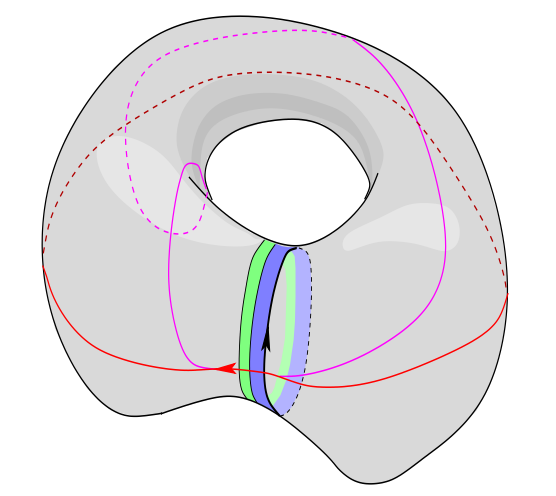
\includegraphics{assets/HarmonicDifferential.png}
    \caption{Source: Figure 3.1 from \cite{Ber06}.
    The black curve $\gamma$ is an arbitrary cycle used to define a harmonic differential. We can define a function $f_\gamma$ that is 1 on the blue belt, 0 outside of the colored belts, and smoothly connects 0 to 1 on the green belt. The exterior derivative $df_\gamma=dh+\eta_\gamma$ lets us identify the harmonic differential $\eta_\gamma$ corresponding to the cycle $\gamma$.}
    \label{figB12:Harmonic}
\end{figure}

\subsection{Definition of Abel's map}

Now that the normalized holomorphic differentials are identified, we can all $g$ of them to produce a function that outputs a $\mathbb C^g$ vector. Since the differentials have known integrals on $a$-cycles and $b$-cycles, the definition of the function can just be made on the fundamental domain, with further points being identified through the cycles.

\begin{definition}[Abel's map]\label{defB12:AbelMap}
    Given the normalized differentials $\omega_i$ for a Riemann surface $\mathcal M$ of genus $g$, we can define Abel's map on the fundamental domain $\mathcal L$ for some chosen basepoint $P_0$
    \begin{align}
        \mathbf{u} : & \ \mathcal L \rightarrow \mathbb C^g \\ & \ P \mapsto \begin{pmatrix}\int_{P_0}^P \omega_1 \\ \vdots \\ \int_{P_0}^P \omega_g \end{pmatrix}.
    \end{align}
    Such a mapping is well defined on the fundamental domain since the integration paths are limited to being homotopically equivalent. We can analytically continue Abel's map to beyond the fundamental domain using known results for integrations along $a$-cycles and $b$-cycles
    \begin{equation}
        \mathbf{u}(P+a_i) = \mathbf{u}(P) + \begin{pmatrix}\int_{a_i} \omega_1 \\ \vdots \\ \int_{a_i} \omega_g \end{pmatrix} = \mathbf{u}(P) + \begin{pmatrix} \delta_{i1} \\ \vdots \\ \delta_{ig} \end{pmatrix},
    \end{equation}
    \begin{equation}
        \mathbf{u}(P+b_i) = \mathbf{u}(P) + \begin{pmatrix}\int_{b_i} \omega_1 \\ \vdots \\ \int_{b_i} \omega_g \end{pmatrix} = \mathbf{u}(P) + \begin{pmatrix} \tau_{i1} \\ \vdots \\ \tau_{ig} \end{pmatrix}.
    \end{equation}
\end{definition}

The simplest example of Abel's map is one we had implicitly already seen before. At genus 1, we can use the familiar cover in which the torus is mapped to the complex plane, where the fundamental domain is a parallelogram with vertices $0$, $1$, $\tau$, $1+\tau$. There is a single holomorphic differential
\begin{equation}
    \omega = dz.
\end{equation}
Using Abel's map, with the basepoint $P_0=0$, we find that
\begin{equation}
    \mathbf{u}(z) = \int_0^z dz = z,\label{eqnB12:AbelGenus1}
\end{equation}
with this result being kept as the map is continued analytically along $a$-cycles and $b$-cycles
\begin{equation}
    \mathbf{u}(P+a_i)=\mathbf{u}(z+1)=\int_0^z dz + \delta_{11} = z+1,
\end{equation}
\begin{equation}
    \mathbf{u}(P+b_i)=\mathbf{u}(z+\tau)=\int_0^z dz + \tau_{11} = z+\tau.
\end{equation}

\begin{figure}
    \center
    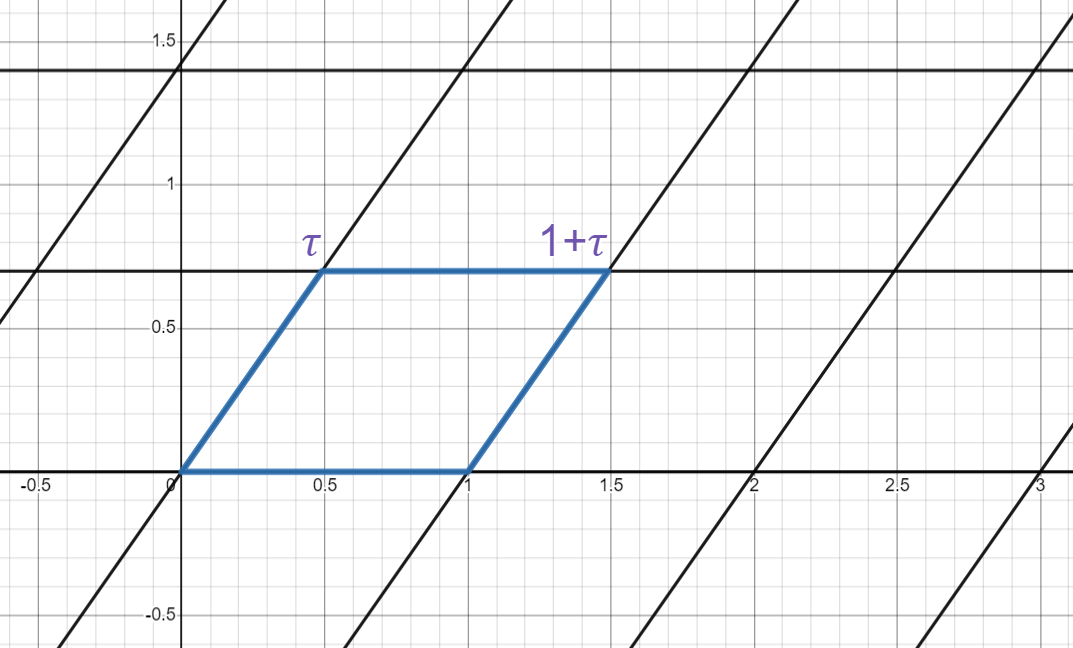
\includegraphics[width=0.6\textwidth]{assets/Domain.png}
    \caption{The fundamental domain at genus 1. Due to the trivial differential $\omega = dz$, we find that Abel's map at genus 1 is simply $\mathbf{u}(z)=z$, justifying the choice of cover.}
\end{figure}

Unfortunately, it is not so simple to define a fundamental domain and identify holomorphic differentials for higher genus. The resolution to this challenge is covered in Section \ref{secB12:SchottkyDifAndAbel}.

\section{Theta functions}\label{secB12:theta}

With Abel's map, we have derived a additively quasiperiodic function that takes us from the manifold to vectors in $\mathbb C^g$. We seek to take advantage of this definition to find a function that instead embodies multiplicative quasiperiodicity. Then, the location of zeros on the Riemann surface will be homotopically invariant, since moving along a cycle and multiplying by some factor will not change whether the function vanishes.

The multiplicative quasiperiodicity will be facilitated by using properties of the exponential function, using the following notation to simplify some expressions
\begin{equation}
    \bolde(z) = \exp(2\pi i z), \quad \bolde(z+1)=\bolde(z).
\end{equation}

\subsection{Definition on $\mathbb C^g$}

\begin{definition}[Theta function]
    Given a $g \times g$ matrix $\tau$ that is symmetric $(\tau = \tau^T)$ and has positive definite imaginary part $(\vec n^T (\Im \tau) \vec n > 0 \forall \vec n \in \mathbb R^g \setminus \vec 0)$, we can define the associated theta function
    \begin{equation} \label{eqnB12:thetaGeneralDefn}
        \Theta(\vec z,\tau) := \sum_{\vec n \in \mathbb Z^g} \bolde\left(\frac{1}{2} \vec n^T \tau \vec n + \vec n^T \vec z\right)
    \end{equation}
    where $\vec z \in \mathbb C^g$. From this point forward the theta functions explicit dependence on $\tau$ will be omitted, since the theta functions are almost always discussed in the context of a $\tau$ chosen to be a constant.
\end{definition}

Though we will omit a formal proof thereof, it is apparent that the series will converge due to the matrix $\tau$ having a positive definite imaginary part supressing terms with large $\vec n$. As we will go on to see in the following section, the choices made for the theta function are made to fit naturally with the formalism we developed for Riemann surfaces, as the matrix $\tau$ will be filled by the period matrix and the input $\vec z$ will be the output of Abel's map.

\begin{lemma}[Properties of the theta function]
    \label{lemmaB12:thetaGeneralProperties}
    The theta function satisfies the properties
    \begin{equation} \label{eqnB12:thetaGeneralEven}
        \Theta(\vec z) = \Theta(-\vec z)
    \end{equation}
    \begin{equation} \label{eqnB12:thetaGeneralShift}
        \Theta(\vec z+\vec \alpha) = \Theta(\vec z) \quad \forall \vec \alpha \in \mathbb Z^g
    \end{equation}
    \begin{equation} \label{eqnB12:thetaGeneralTauShift}
        \Theta(\vec z + \tau \vec \beta) = \bolde\left(-\frac{1}{2}\vec \beta^T \tau \vec \beta - \vec \beta^T \vec z\right) \Theta(\vec z) \quad \forall \vec \beta \in \mathbb Z^g
    \end{equation}
\end{lemma}

\begin{proof} The simple proofs of the three properties are included for the convenience of the reader.

    Proving that the theta function is even (\ref{eqnB12:thetaGeneralEven})
    \begin{align}
        \Theta(-\vec z) = \sum_{\vec n \in \mathbb Z^g} \bolde\left(\frac{1}{2} \vec n^T \tau \vec n + \vec n^T (-\vec z)\right) \overset{\vec n \mapsto -\vec m}{=} \sum_{\vec m \in \mathbb Z^g} \bolde\left(\frac{1}{2} \vec m^T \tau \vec m + \vec m^T \vec z\right) = \Theta(\vec z)
    \end{align}
    Proving that the theta function is invariant under integer shifts (\ref{eqnB12:thetaGeneralShift})
    \begin{align}
        \Theta(\vec z + \vec \alpha) &= \sum_{\vec n \in \mathbb Z^g} \bolde\left(\frac{1}{2} \vec n^T \tau \vec n + \vec n^T (\vec z + \vec \alpha)\right) \\ &=
        \sum_{\vec n \in \mathbb Z^g} \underset{=1}{\underbrace{\bolde\left(\vec n^T \vec \alpha\right)}} \bolde\left(\frac{1}{2} \vec n^T \tau \vec n + \vec n^T \vec z\right) = \Theta(\vec z)
    \end{align}
    Proving that the theta function is invariant under period matrix shifts (\ref{eqnB12:thetaGeneralTauShift})
    \begin{align}
        \Theta(\vec z + \tau \vec \beta) &= \sum_{\vec n \in \mathbb Z^g} \bolde\left(\frac{1}{2} \vec n^T \tau \vec n + \vec n^T (\vec z + \tau \vec \beta)\right) \\ &=
        \sum_{\vec n \in \mathbb Z^g}
        \bolde\left(-\frac{1}{2} \vec \beta^T \tau \vec \beta - \vec \beta^T \vec z\right) \bolde\left(\frac{1}{2} (\vec n+\vec \beta)^T \tau (\vec n+\vec \beta) + (\vec n+\vec \beta)^T \vec z\right)\\
        &=  \bolde\left(-\frac{1}{2} \vec \beta^T \tau \vec \beta - \vec \beta^T \vec z\right) \Theta(\vec z) 
    \end{align}
\end{proof}

\subsection{Definition on compact Riemann surface}
Now, we can combine Abel's map (\ref{defB12:AbelMap}) and the theta function above (\ref{eqnB12:thetaGeneralDefn}) to identify theta functions directly on a compact Riemann surface. The properties of the two functions work perfectly together to produce desired quasiperiodic results on the Riemann surface.

\begin{definition}[Theta function on a compact Riemann surface]
    Using Abel's map $\mathbf{u} : \mathcal M \mapsto \mathbb C^g$ with some basepoint $P_0 \in \mathcal M$, and the theta function $\Theta : \mathbb C^g \mapsto \mathbb C$ with $\tau$ corresponding to the period matrix of $\mathcal M$, we identify

    \begin{equation}
        \theta(P) = \Theta(\mathbf{u}(P),\tau)
    \end{equation}
    as a theta function on the Riemann surface.
\end{definition}

\begin{lemma}[Properties of theta functions on a compact Riemann surface]
    Using the analytic continuation provided by Abel's map and the quasiperiodic properties of the theta function, we find that
    \begin{equation}
        \theta(P+a_i) = \theta(P),
    \end{equation}
    \begin{equation}
        \theta(P+b_i) = \bolde\left(-\mathbf{u}_i(P)-\frac{1}{2}\tau_{ii}\right)\theta(P).
    \end{equation}
\end{lemma}

Recall that Abel's map on a genus 1 Riemann surface is simply $\mathbf{u}(z)=z$ (Equation \ref{eqnB12:AbelGenus1}). We can then easily see that the theta function on a genus 1 Riemann surface is simply
\begin{equation}
    \theta(z) = \Theta(\mathbf{u}(z)) = \Theta(z) = \sum_{n \in \mathbb Z} \bolde\left(\frac{1}{2}n^2 \tau + n z\right),
\end{equation}
a plot of which is seen in Figure \ref{figB12:Genus1theta}.

\begin{figure}
    \center
    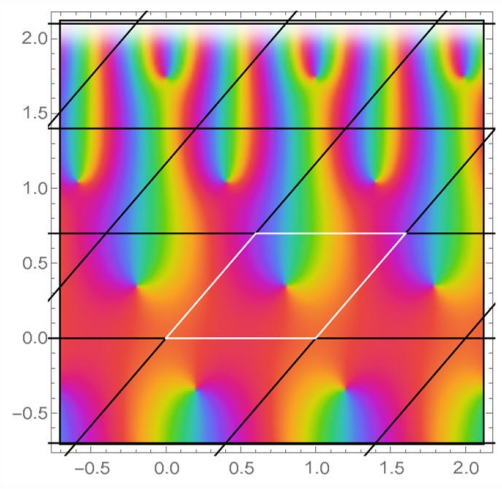
\includegraphics{assets/genus1theta.png}
    \caption{Source: \cite{Cha22}.
    Complex plot of the theta function on a genus 1 surface with $\tau = 0.7+0.6i$. For $\theta(z)=r\exp(i\phi)$, the color represents the argument $\phi$. One can see the quasiperiodic properties: the plot is perfectly symmetric with respect to shifts by 1 ($a$-cycles), and quasiperiodic with respect to shifts by $\tau$ ($b$-cycles). The points around which the color wraps are simple zeros, the locations of which are proven in Theorem \ref{thmB12:OddLocations}.}
    \label{figB12:Genus1theta}
\end{figure}

\subsection{Characteristics and zeros}
\begin{definition}[Theta function with characteristics]
    For vectors $\epsilon,\epsilon' \in \mathbb C^g$, the theta function with characteristics is defined as
    \begin{align}
        \Theta\begin{bmatrix} \epsilon \\  \epsilon'\end{bmatrix}(\vec z) :=& \ 
        \bolde\left(\frac{1}{8}\epsilon^T \tau \epsilon + \frac{1}{2}\epsilon^T \vec z + \frac{1}{4}\epsilon^T  \epsilon'\right)
        \Theta\left(\vec z + \frac{\epsilon'}{2}+\frac{\tau\epsilon}{2}\right)
       \\ =& \sum_{\vec n \in \mathbb Z^g} \bolde\left(\frac{1}{2} (\vec n+\epsilon/2)^T \tau (\vec n+\epsilon/2) + (\vec n+\epsilon/2)^T (\vec z+\epsilon'/2)\right).
    \end{align}

    Note that many sources (e.g. \cite{Cha22} and \cite{ComputationalSchottky}) use $\epsilon,\epsilon' \mapsto \epsilon/2,\epsilon'/2$ instead to simplify parts of the notation.
\end{definition}

The choice of adding characteristics to the theta functions in this way seems arbitrary, but it actually leads to a few key properties. First, it is apparent from the definition that the theta function, and consequently its zeros, are shifted by some controlled amount. Second, the quasiperiodicity and parity properties of the theta function will change in ways that we will be able to take advantage of.

\begin{lemma}[Properties of the theta functions with characteristics]
    The theta function satisfies the properties
    \begin{equation}\Theta\begin{bmatrix}\epsilon \\ \epsilon'\end{bmatrix}(\vec z + \vec \alpha + \tau \vec \beta) =
    \ee\left(\frac{1}{2}(\epsilon^T \vec \alpha - \vec \beta^T \epsilon') - \frac{1}{2} \beta^T \tau \beta - \vec \beta \vec z\right)
    \Theta\begin{bmatrix}\epsilon \\ \epsilon'\end{bmatrix}(\vec z)
    \end{equation}

    \begin{equation}\Theta\begin{bmatrix}\epsilon + 2\eta \\ \epsilon' + 2\eta' \end{bmatrix}(\vec z) = \exp(\pi i \epsilon^T \eta')
    \Theta\begin{bmatrix}\epsilon \\ \epsilon'\end{bmatrix}(\vec z) , \quad \eta,\eta' \in \mathbb Z^g\end{equation}
    % \pause
    \begin{equation}\Theta\begin{bmatrix}\epsilon \\ \epsilon'\end{bmatrix}(-\vec z) = \exp(\pi i \epsilon^T \epsilon') \Theta\begin{bmatrix}\epsilon \\ \epsilon'\end{bmatrix}(\vec z) , \quad \epsilon,\epsilon' \in \mathbb Z^g\end{equation}

    The first property is analogous to the quasiperiodicity of the theta function before (\ref{eqnB12:thetaGeneralShift} and \ref{eqnB12:thetaGeneralTauShift}).
    
    The second property shows that, up to a sign, the characteristics are equivalent modulo 2.
    
    The third property defines the parity of the resulting theta function; note that it is only true for integer characteristics.
\end{lemma}

\begin{proof}
    The first and second properties are proved analogously to Lemma \ref{lemmaB12:thetaGeneralProperties}.

    The third property uses
    \begin{equation}
        \Theta\begin{bmatrix}\epsilon \\ \epsilon'\end{bmatrix}(\vec z) = \Theta\begin{bmatrix}-\epsilon \\ -\epsilon'\end{bmatrix}(-\vec z)
    \end{equation}
    followed by applying the second property using $\eta=2\epsilon$ and $\eta=2\epsilon'$ to return to the original characteristics with a possible sign difference.
\end{proof}

The third property tells us that for characteristics $\epsilon,\epsilon' \in \mathbb Z^g$ such that $\epsilon^T\epsilon'$ is odd, the resulting theta function will be odd. Since odd function vanish at the origin, this property can be used to identify the locations of zeros for the theta function in general.

\begin{theorem}[Location of zeros of the theta function]\label{thmB12:OddLocations}
    The zeros of the theta function are
    \begin{equation}
        \Theta\left(\frac{\epsilon}{2} + \frac{\tau \epsilon'}{2}\right) = 0
    \end{equation}
    for all $\epsilon,\epsilon' \in \mathbb Z^g$ for which $\epsilon^T \epsilon'$ is odd.
\end{theorem}

\begin{proof}
    For such $\epsilon$ and $\epsilon'$, we find that
    \begin{equation}
        \Theta\begin{bmatrix}\epsilon \\ \epsilon'\end{bmatrix}(-\vec z) = -\Theta\begin{bmatrix}\epsilon \\ \epsilon'\end{bmatrix}(\vec z) \implies \Theta\begin{bmatrix}\epsilon \\ \epsilon'\end{bmatrix}(0) = 0.
    \end{equation}
    Using the definition of the theta function with characteristics
    \begin{equation}
        \Theta\begin{bmatrix}\epsilon \\ \epsilon'\end{bmatrix}(0) = \overset{\neq 0}{\overbrace{\bolde( \cdots )}}\Theta\left(0+ \frac{\epsilon'}{2}+\frac{\tau\epsilon}{2}\right) = 0,
    \end{equation}
    we find that
    \begin{equation}
        \Theta\left(\frac{\epsilon'}{2}+\frac{\tau\epsilon}{2}\right) = 0
    \end{equation}
    as desired.
\end{proof}

Depending on the genus, the number of possible odd characteristics changes. Indeed, one can prove that the precise number is $2^{g-1}(2^g-1)$ choices out of the $2^{2g}$ possible integer characteristics modulo 2. At genus 1, this leaves only a single function, known as \emph{the} odd theta function at genus 1.

\begin{definition}[The odd theta function at genus 1]
    The odd theta function at genus 1 can be identified as
    \begin{equation}
        \theta_1(z) = -\Theta \begin{bmatrix}1 \\ 1\end{bmatrix} (z),
    \end{equation}
    where the choice of characteristics $\epsilon=\epsilon'=1$ is the only possible odd choice, and the extra $-1$ factor exists by convention.
\end{definition}

\subsection{Decomposition of functions}\label{secB12:decomposition}
To provide some intuition and illustration of the properties of theta functions, this section will describe their use in the decomposition of meromorphic functions.

Parts of this proof have already been done in \ref{rep:A5}, with results for decompositions of meromorphic functions at genus 0 (Equation \ref{eqnA5:eqnA5:rational product}) and at genus 1 (Equation \ref{eqnA5:trans-theta-ratio}).

Consider decomposing a function $f$ with divisor $(f)$ (see \ref{rep:A9} for an overview of divisors). We can approach this by constructing a function $g$ such that $(g)=(f)$. Then, the function $f/g$ has divisor $(f/g)=(f)-(g)=0$, and is thus constant by Liouville's theorem (Theorem \ref{thrmA9:1_Liouville_compact_surface}). Consequently, the desired function $f$ is off from our constructed function $g$ by a constant.

\begin{lemma}[Decomposition at genus 0]
    Given a function $f$ on the Riemann sphere, with divisor $(f)=\sum_i n_i z_i$, it can be decomposed as
    \begin{equation}
        f = c \prod_i (z-z_i)^n_i.
    \end{equation}
\end{lemma}

\begin{lemma}[Decomposition at genus 1]
    Consider a function $f$ on the Torus, with divisor $(f) = \sum_i n_i z_i$. If we decompose $z_i = b_i/2 + \tau a_i/2$, then we can write
    \begin{equation}
        f = c \prod_i \left[\Theta\begin{bmatrix}a_i+1 \\ b_i+1\end{bmatrix}(z)\right]^{n_i}.
    \end{equation}
    The result will indeed be elliptic through a cancellation of quasiperiodic factors \cite{Cha22}, though the proof of this is beyond the scope of this report.
\end{lemma}

\begin{lemma}[Decomposition at arbtirary genus $\geq 1$]
    Choosing $\vec e$ such that $\Theta(\vec e)=0$ \cite{Ber06}, we can decompose the hyperelliptic function $f$ with divisor $(f) = \sum_i n_i P_i$ as 
    \begin{equation}
        f(P) = c \prod_i \left[\Theta(\mathbf{u}(P) - \mathbf{u}(P_i) + \vec e)\right]^{n_i}.
    \end{equation}
\end{lemma}

Essentially, we can see the theta functions as higher genus analogues of a linear monomial. This will come into play to inspire the choice of the Kronecker function in the next section.

\section{Kronecker function}\label{secB12:Kronecker}

With a better understanding and formalism of theta functions, we can now return to the Kronecker function from prior reports (\ref{rep:B10} and \ref{rep:B11}). Rather than focusing on the consequences that the Kronecker function has for multiple elliptic polylogarithms \cite{BL13} or its applications to string theory \cite{Broedel_2022}, we will focus on the properties that it has and how those properties are inherited by the functions used in its expansion.

\subsection{Genus 0 analogy}

At genus 0, the multiple polylogarithms are generated using the differentials
\begin{equation}
    g^{(0)}(z)dz = 1 dz , \quad g^{(1)}(z)dz = \frac{1}{z} dz.
\end{equation}

One way to make them appear is by noting that from the function
\begin{equation}
    \tilde F(z,\alpha) = \frac{z+\alpha}{z\alpha},
\end{equation}
once it is expanded in $\alpha$
\begin{equation}\label{eqnB12:ExpandExample}
    \alpha \tilde{F}(z,\alpha) = \alpha^0 g^{(0)}(z) + \alpha^1 g^{(1)}(z),
\end{equation}
we find the two differentials as coefficients of the powers.

Furthermore, with some effort we can identify that
\begin{equation}
    \tilde{F}(z_1,\alpha_1)\tilde{F}(z_2,\alpha_2) = \tilde{F}(z_1,\alpha_1+\alpha_2)\tilde{F}(z_2-z_1,\alpha_2) + \tilde{F}(z_2,\alpha_1+\alpha_2)\tilde{F}(z_1-z_2,\alpha_1),
\end{equation}
which is the titular \emph{bilinear relation}. In the next section with the actual Kronecker function, the analogous relation will be called the Fay identity.

Expanding this relation as done in Equation \ref{eqnB12:ExpandExample} and matching corresponding powers of $\alpha_i$ will give us the result
\begin{equation}
    g^{(1)}(z_1)g^{(1)}(z_2) = g^{(1)}(z_1)g^{(1)}(z_2-z_1) + g^{(1)}(z_2)g^{(1)}(z_1-z_2),
\end{equation}
which is more easily recognized as a partial fraction identity with $z_1 \mapsto (t-a)$ and $z_2 \mapsto (t-b)$
\begin{equation}
    \frac{1}{(t-a)(t-b)} = \frac{1}{(t-a)(a-b)} + \frac{1}{(t-b)(b-a)},
\end{equation}
which has uses for evaluating integral representations of multiple polylogarithms \cite{Broedel_2015}.

Of course, proving this relation for partial fractions does not require the roundabout way using the function $\tilde F$. However, this example is representative of what is done for genus 1.

\subsection{Definition and properties of the Kronecker function}

In section \label{secB12:decomposition}, we showed how theta functions are analogous to linear monomials through the way meromorphic functions are decomposed at various genera. In the previous section, we used linear monomials in order to construct $\tilde F$ which generated differentials $g^{(i)}$ useful for multiple polylogarithms \cite{rep:B1}. Combining these ideas, we can define the Kronecker function $F$, using the odd theta function at genus 1 instead of linear monomials.

\begin{definition}[The Kronecker function]
    The Kronecker function $F(z,\alpha,\tau)$ has equivalent definitions
    \begin{enumerate}
        \item In terms of the odd theta function
        \begin{equation}\frac{\theta_1'(0)\theta_1(z+\alpha)}{\theta_1(z)\theta_1(\alpha)}\end{equation}
        \item In terms of a sum over exponentials
        \begin{equation}-2\pi i \left(\frac{z}{1-z} + \frac{1}{1-w} + \sum_{m,n > 0} (z^m w^n - z^{-m} w^{-n}) q^{mn}\right) , \quad \begin{pmatrix} z \\ w \\ q \end{pmatrix} = \bolde \begin{pmatrix}\xi \\ \alpha \\ \tau\end{pmatrix}\end{equation}
        \item In terms of a sum over Eisenstein functions and series
        \begin{equation}\frac{1}{\alpha} \exp\left(-\sum_{j > 0} \frac{(-\alpha)^j}{j} (E_j(z,\tau) - e_j(\tau))\right)\end{equation}
    \end{enumerate}
    where $E_j(z,\tau)$ and $e_j(\tau)$ are the Eisenstein functions and series, defined by
    \begin{equation}
        E_j(\xi,\tau) = \lim_{N,M\rightarrow \infty} \sum_{n=-N}^N \sum_{m=-M}^M \frac{1}{(\xi+m+n\tau)^j}, \quad e_j(\tau) = \lim_{N,M\rightarrow \infty} \underset{\mathrm{except \ }(m,n)=(0,0)}{\underbrace{\sum_{n=-N}^N \sum_{m=-M}^M}} \frac{1}{(m+n\tau)^j}.
    \end{equation}

    The Kronecker function satisfies quasiperiodic relations in the first variable
    \begin{equation}
        F(z+1,\alpha)=F(z,\alpha),
    \end{equation}
    \begin{equation}
        F(z+\tau,\alpha)=\bolde(-\alpha)F(z,\alpha).
    \end{equation}
\end{definition}

\begin{proof}
    An complete outline of the proof of equivalence of the definitions is given in \cite{BL13}.

    The quasiperiodicity can be proved using the first definition and the quasiperiodicity of the theta function
    \begin{equation}
        F(z+1,\alpha) = \frac{\theta'(0)\theta(z+\alpha+1)}{\theta(z+1)\theta(\alpha)} = \frac{\theta'(0)\theta(z+\alpha)}{\theta(z)\theta(\alpha)} = F(z,\alpha)
    \end{equation}
    \begin{equation}
        F(z+\tau,\alpha) = \frac{\theta'(0)\theta(z+\alpha+\tau)}{\theta(z+\tau)\theta(\alpha)} = \frac{\bolde(-z-\alpha)\theta'(0)\theta(z+\alpha)}{\bolde(-z)\theta(z)\theta(\alpha)} = \bolde(-\alpha) F(z,\alpha)
    \end{equation}
\end{proof}

\begin{lemma}[The Fay identity]
    The Kronecker function defined above satisfies
    \begin{equation}\label{eqnB12:FayKronecker}
        {F}(z_1,\alpha_1){F}(z_2,\alpha_2) = {F}(z_1,\alpha_1+\alpha_2){F}(z_2-z_1,\alpha_2) + {F}(z_2,\alpha_1+\alpha_2){F}(z_1-z_2,\alpha_1).
    \end{equation}
\end{lemma}

\begin{proof}
    A complete outline of the proof is given in \cite{Mat19} and is paraphrased here.

    Using the definition of the Kronecker function in terms of theta functions, we can multiply by all the denominators.
    This gives us three terms, each of which is a product of 4 theta functions. After a relabeling of their arguments, we reach
    \begin{align}
        & \theta_1(a_0)\theta_1(b_0)\theta_1(a_2+b_1)\theta_1(a_2-b_1) + \\
        & \theta_1(a_1)\theta_1(b_1)\theta_1(a_0+b_2)\theta_1(a_0-b_2) + \\
        & \theta_1(a_2)\theta_1(b_2)\theta_1(a_1+b_0)\theta_1(a_1-b_0) = 0,
    \end{align}
    which has convenient symmetry properties. We can conclude the proof by noting that this is Proposition 5 from \cite{Zagier1991}.
\end{proof}

\subsection{Decomposition of the Kronecker function}

With the Kronecker function defined, we can now take an expansion in $\alpha$ to recover appropriate differentials. Unlike the analogous genus 0 case (Equation \ref{eqnB12:ExpandExample}), there will be an infinite tower of differentials.

\begin{definition}[Holomorphic functions from the Kronecker function]
    Expanding the Kronecker function in powers of $\alpha$
    \begin{equation}
        \alpha F(z,\alpha) = \sum_{n=0}^{\infty} g^{(n)}(z) \alpha^n,
    \end{equation}
    we find the functions $g^{(n)}(z)$, which are suitable integration kernels for elliptic polylogarithms (\ref{rep:B10}) \cite{Broedel_2022}.
\end{definition}

The resulting functions have power expansions in $q = \bolde(\tau)$ \cite{Broedel_2015}
\begin{equation}
    g^{(0)}(z) = 1,
\end{equation}
\begin{equation}
    g^{(1)}(z) = \pi \cot(\pi z) + 4 \pi \sum_{m=1}^\infty \sin(2 \pi m z) \sum_{n=1}^\infty q^{mn},
\end{equation}
\begin{equation}
    g^{(k)}(z)\big|_{k=2,4,\ldots} = -2\left[\xi_k + \frac{(2\pi i)^k}{(k-1)!} \sum_{m=1}^\infty \cos(2 \pi m z) \sum_{n=1}^\infty n^{k-1} q^{mn} \right],
\end{equation}
\begin{equation}
    g^{(k)}(z)\big|_{k=3,5,\ldots} = -2i \frac{(2\pi i)^k}{(k-1)!} \sum_{m=1}^\infty \sin(2\pi mz) \sum_{n=1}^\infty n^{k-1} q^{mn}.
\end{equation}

We can also easily deduce the parity of these functions,
\begin{equation}
    \theta_1(z) = -\theta_1(-z) \implies F(z,\alpha) = -F(-z,-\alpha) \implies g^{(n)}(z)=(-1)^n g^{(n)}(-z).
\end{equation}


Using the Fay identity for the Kronecker function (\ref{eqnB12:FayKronecker}), we can prove a relation for the functions that it expanded to.

\begin{lemma}[Fay identity satisfied by expansion of the Kronecker function]
    The functions $g^{(n)}$ from the expansion of the Kronecker function in the second variable satisfy
    \begin{align}
        g^{(m)}(z_1) g^{(n)}(z_2) = (-1)^{n-1} g^{(m+n)}(z_1-z_2)& \\
         +\sum_{r=0}^n \begin{pmatrix} m+r-1 \\ r \end{pmatrix} g^{(m+r)}(z_1) g^{(n-r)}(z_2-z_1) & \\
         +\sum_{r=0}^m \begin{pmatrix} n+r-1 \\ r \end{pmatrix} g^{(n+r)}(z_2) g^{(m-r)}(z_1-z_2) & .
    \end{align}
\end{lemma}

\begin{proof}
    We begin by expanding each Kronecker function in their Fay identity
    \begin{equation}
        {F}(z_1,\alpha_1){F}(z_2,\alpha_2) = {F}(z_1,\alpha_1+\alpha_2){F}(z_2-z_1,\alpha_2) + {F}(z_2,\alpha_1+\alpha_2){F}(z_1-z_2,\alpha_1)
    \end{equation}
    \begin{align}
        \implies & \left(\frac{1}{\alpha_1} \sum_{j=0}^{\infty} g^{(j)}(z_1) \alpha_1^j\right)
        \left(\frac{1}{\alpha_2} \sum_{j=0}^{\infty} g^{(j)}(z_2) \alpha_2^j\right) =
        \\ & \quad \quad \left(\frac{1}{\alpha_1+\alpha_2} \sum_{j=0}^{\infty} g^{(j)}(z_1) (\alpha_1+\alpha_2)^j\right)
        \left(\frac{1}{\alpha_2} \sum_isolate {j=0}^{\infty} g^{(j)}(z_2-z_1) \alpha_2^j\right) +
        \\ & \quad \quad \left(\frac{1}{\alpha_1+\alpha_2} \sum_{j=0}^{\infty} g^{(j)}(z_2) (\alpha_1+\alpha_2)^j\right)
        \left(\frac{1}{\alpha_1} \sum_{j=0}^{\infty} g^{(j)}(z_1-z_2) \alpha_1^j\right).
    \end{align}

    Then, multiplying through by $\alpha_1\alpha_2(\alpha_1+\alpha_2)$ to remove fractions, we can isolate the coefficients of $\alpha_1^n \alpha_2^m$ and find
    \begin{align}
        & g^{(m-1)}(z_1)g^{(n)}(z_2)+g^{(m)}(z_1)g^{(n-1)}(z_2) = \label{eqnB12:kernelFaySTART}
        \\ & \quad \quad \sum_{j=0}^{n} \begin{pmatrix} m-1+j \\ j \end{pmatrix} g^{(m-1+j)}(z_1) g^{(n-j)}(z_2-z_1) +
        \\ & \quad \quad \sum_{j=0}^{m} \begin{pmatrix} n-1+j \\ j \end{pmatrix} g^{(n-1+j)}(z_2) g^{(m-j)}(z_1-z_2),
    \end{align}
    as in Equation 3.29 of \cite{Broedel_2015}.

    By relabeling $m \mapsto m+1$, and isolating the resulting $g^{(m)}(z_1)g^{(n)}(z_2)$ term, we can use a careful proof by induction involving combinatorics to show that
    \begin{align}
        g^{(m)}(z_1) g^{(n)}(z_2) = (-1)^{n-1} g^{(m+n)}(z_1-z_2)& \\
         +\sum_{r=0}^n \begin{pmatrix} m+r-1 \\ r \end{pmatrix} g^{(m+r)}(z_1) g^{(n-r)}(z_2-z_1) & \\
         +\sum_{r=0}^m \begin{pmatrix} n+r-1 \\ r \end{pmatrix} g^{(n+r)}(z_2) g^{(m-r)}(z_1-z_2) & .
    \end{align}

    The details of this cumbersome last step are contained in Appendix \ref{appB12:kernelFay}.
\end{proof}

\subsection{Perfectly periodic differentials and their independence}

In some applications, it is more useful to have the expansion produce functions that are perfectly periodic, sacrificing holomorphicity.
Recall that this sacrifice is necessary, since it is not possible to have non-constant holomorphic and perfectly periodic functions.

\begin{definition}[Perfectly periodic differential and expansion]
    We define a differential from the Kronecker function that is perfectly periodic in the first argument as
    \begin{equation}
        \Omega(z,\alpha) = \bolde\left( \alpha \frac{\Im(z)}{\Im(\tau)}\right) F(z,\alpha) dz.
    \end{equation}

    The exterior derivative of this differential is
    \begin{equation}
        d\Omega(z,\alpha) = \nu \alpha \wedge \Omega(z,\alpha),
    \end{equation}
    for $\nu = 2 \pi i \cdot d\!\left(\frac{\Im(z)}{\Im(\tau)}\right)$.

    Analogously to the Kronecker function, we can do an expansion in $\alpha$
    \begin{equation}
        \alpha \Omega(z,\alpha) = \sum_{n=0}^\infty f^{(n)}(z) \alpha^n,
    \end{equation}
    giving perfectly periodic differentials $f^{(n)}(z)$.
\end{definition}

\begin{proof}
    We can easily show the periodicity properties of $\Omega$,
    \begin{equation}
        \Omega(z+1,\alpha) = \bolde\left( \alpha \frac{\Im(z+1)}{\Im(\tau)}\right) F(z+1,\alpha) dz = \bolde\left( \alpha \frac{\Im(z)}{\Im(\tau)}\right) F(z,\alpha) dz = \Omega(z,\alpha),
    \end{equation}
    \begin{equation}
        \Omega(z+\tau,\alpha) = \bolde\left( \alpha \frac{\Im(z+\tau)}{\Im(\tau)} \right) F(z+\tau,\alpha) dz = \bolde\left( \alpha \frac{\Im(z)}{\Im(\tau)}\right) \bolde(\alpha) \bolde(-\alpha) F(z,\alpha) dz = \Omega(z,\alpha).
    \end{equation}
\end{proof}

\begin{lemma}[Independence of differentials]
    The differentials $\{f^{(n)}$ for $n \geq 0\}$ from the expansion of $\Omega$ are linearly independent over $\mathbb C$.
\end{lemma}
\begin{proof}
    This proof is a paraphrased version of one found in \cite{BL13}.

    The relation $d\Omega = \nu \wedge \Omega$ gives us that
    \begin{equation}
        df^{(n+1)} = \nu \wedge f^{(n)} \quad \forall n > 0,
    \end{equation}
    which can be completed by noting
    \begin{equation}
        df^{(0)} = d^2 z = 0.
    \end{equation}

    TO DO: REST OF PROOF

\end{proof}

\section{Schottky Covers}\label{secB12:Schottky}

With an understanding of the Kronecker function at genus 1, we may ask how one can approach working with higher genus surfaces.
The first hurdle to overcome is that of creating a suitable cover, on which we can begin to define our analytical tools, like holomorphic differentials.

We can approach this by constructing covers in which $a$-cycles are represented by circles in the complex plane \cite{ComputationalSchottky} \cite{Cha22}.

\subsection{Definition of the Schottky group and cover}
In order to create maps involving discs on the complex plane, we can use Mobius transformations.

\begin{definition}[Mobius transformations]
    A Mobius transformation $\gamma$ is a meromorphic map on the Riemann sphere $\mathbb C \cup \{\infty\}$ characterized by constants $a,b,c,d \in \mathbb C$
    \begin{equation}
        \gamma : \mathbb C \cup \{\infty\} \rightarrow \mathbb C \cup \{\infty\} ; \ z \mapsto \frac{az+b}{cz+d}
    \end{equation}
    with $ad-bc \neq 0$. Since rescaling of the coefficients $a,b,c,d\mapsto \lambda a,\lambda b, \lambda c, \lambda d$ do not change the map, they can be normalized to $ad-bc=1$.
\end{definition}

These Mobius transformations can then be used to define the Schottky group.
The group is defined by pairs of discs, such that there is a generator for each pair that sends the outside of one disc to the inside of another.
Figure \ref{figB12:MobiusIllustration} depicts how one may construct such a Mobius transformation.

We will find that this is a suitable group for describing a compact Riemann surface. The intuition for why this works may be gleaned from Figure \ref{figB12:SchottkyIntuition}, as the boundaries of the discs will represent $a$-cycles on our surface.

\begin{figure}
    \center
    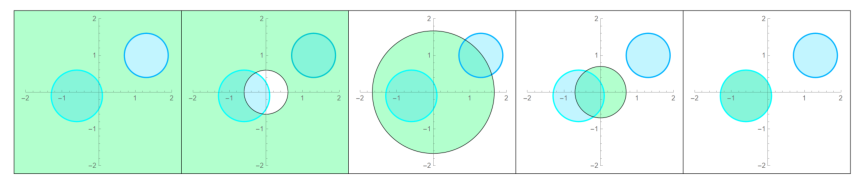
\includegraphics[width=\textwidth]{assets/ChanSchottkyGroup.png}
    \caption{
        Source: \cite{Cha22}.
        An illustration for how a Mobius transformation can be chosen to map the outside of one disc to the inside of another.
        From left to right, we iteratively transform the outside to the inside by:
        shifting to the origin ($z \mapsto z-x_1$), inverting ($z \mapsto 1/z$), rescaling ($z \mapsto r_1r_2 z$), and shifting to the appropriate center ($z \mapsto z+x_2$), 
        where $x_1,x_2$ are the centers and $r_1,r_2$ are the radii of the respective discs.
    }
    \label{figB12:MobiusIllustration}
\end{figure}

\begin{figure}
    \center
    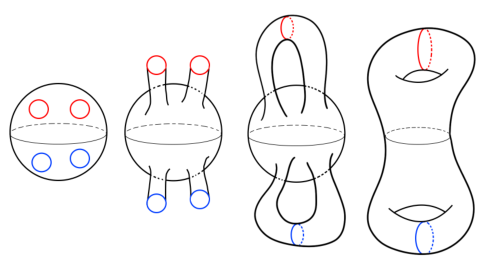
\includegraphics{assets/ChanSchottkyCover.png}
    \caption{
        Source: \cite{Cha22}.
        As we move past an $a$-cycle on the compact Riemann surface (right), we move inside the corresponding disc on the Riemann sphere (left).
        On the Riemann surface, we continue past the $a$-cycle to the other half of the handle it is on.
        On the sphere, this is equivalent to moving outside the other disc in the pair.
        The Schottky group, mapping insides of one disc to the outside of another, puts the structure we expect on the Riemann surface onto the Riemann sphere with discs.
    }
    \label{figB12:SchottkyIntuition}
\end{figure}

\begin{definition}[Schottky group]
    Choosing mutually disjoint discs $\{D_i,D_i'\}$ with interiors $\{\mathring{D}_i,\mathring{D}_i'\}$ on a Riemann sphere,
    we can choose mobius transformations $\gamma_i$ such that the exterior of $D_i$ is mapped to the interior of $D_i'$
    \begin{equation}
        \gamma_i \in \text{PSL}_2(\mathbb C) , \quad \gamma_i : z \mapsto \frac{az+b}{cz+d}
    \end{equation}
    \begin{equation}
        \gamma_i(\bar C \setminus \mathring{D}_i) = D_i'
    \end{equation}
    \begin{equation}
        \gamma_i(\partial D_i) = \partial D_i'
    \end{equation}

    The transformations formed by composition of $\gamma_i$ form the Schottky group $\Gamma$.
\end{definition}

The Schottky group can then be used to represent a Riemann surface.
This process is called the uniformization of a Riemann surface; unfortunately a closer look at this process is beyond the scope of this report.

\begin{definition}[Schottky cover]
    Given a Schottky group $\Gamma$ corresponding to $g$ pairs of discs $\{D_i,D_i'\}$, we can denote
    \begin{equation}
        F = \mathbb C \cup \{\infty\} \setminus \bigcup_i \left( \mathring{D}_i,\mathring{D}_i' \right),
    \end{equation}
    \begin{equation}
        \Omega = \bigcup_{\gamma \in \Gamma} \gamma(F).
    \end{equation}

    Then, $\mathcal M = \Omega / \Gamma$ is a Riemann surface of genus $g$, with fundamental domain $F$.
\end{definition}

Though a step towards the intuition was already seen in Figure \ref{figB12:SchottkyIntuition}, with the proper definition in hand we can take another look.
As we expect, the fundamental domain $F$ is the fundamental domain of the Riemann surface $\mathcal M$, bounded by several of the $a$-cycles.
The Schottky group produces infinite copies of the fundamental domain inside of the discs, as in the formula for $\Omega$.
These copies are entered by any path that crosses one of the chosen $a$-cycles, but is returned to the fundamental domain by the action of a generator of $\Gamma$.
To aid in developing this intuition, Figure \ref{figB12:SchottkyIntuition2} shows the fundamental domain and one of its copies.

\begin{figure}
    \center
    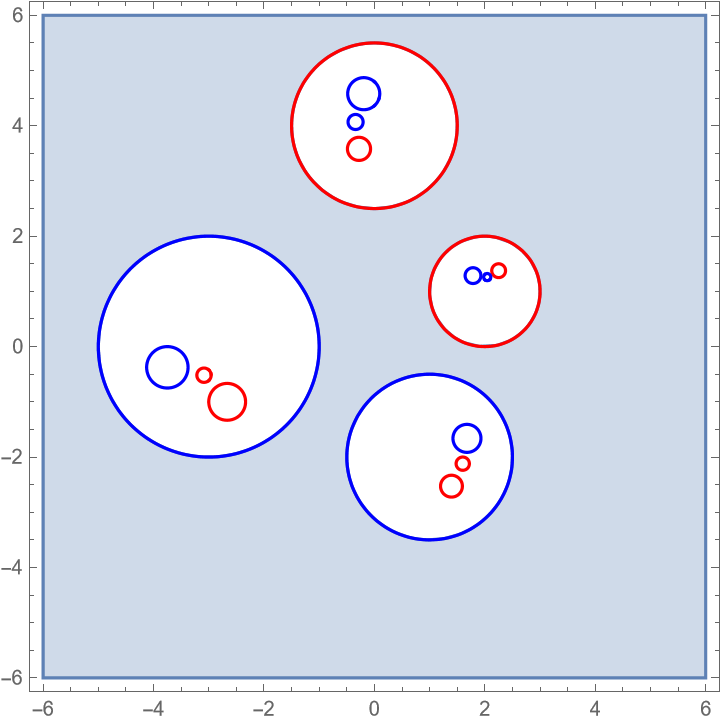
\includegraphics[width=0.4\textwidth]{assets/Genus2SchottkyOuter.png}
    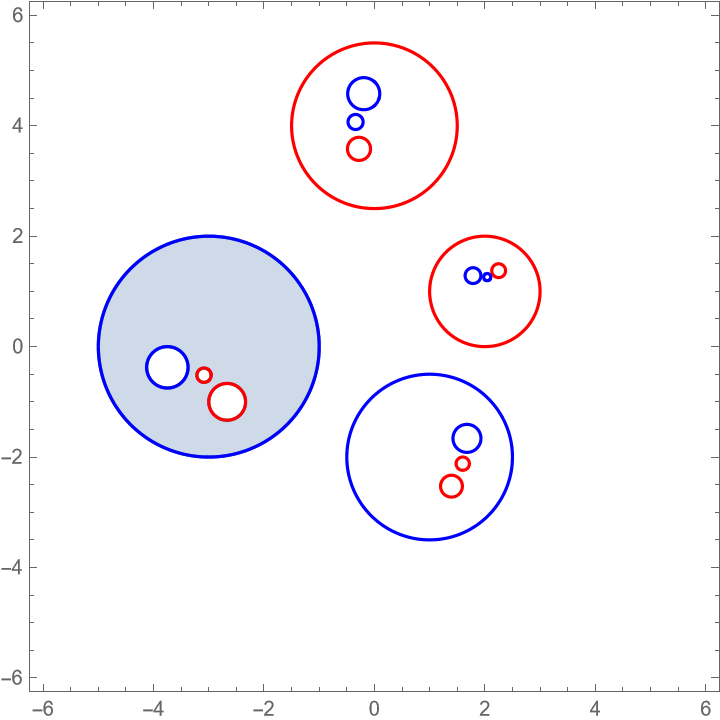
\includegraphics[width=0.4\textwidth]{assets/Genus2SchottkyInner.png}
    \caption{
        Two images of the same Schottky cover for some genus 2 Riemann surface.
        On the left, the fundamental domain is highlighted.
        On the right, an image of the fundamental domain after the action of some element of the Schottky group is highlighted.
    }
    \label{figB12:SchottkyIntuition2}
\end{figure}

\subsection{Differentials and Abel's map}\label{secB12:SchottkyDifAndAbel}

Using the Schottky cover, we can now define the tools we used in Section \ref{secB12:Abel} at higher genus in a practical way.
Though it is not demonstrated in this report, such a step is instructive as it allows us to see directly the consequences of our constructions at higher genera.

In order to properly define the holomorphic differentials and Abel's map in a convergent manner, we must first analyze the fixed points of the generators $\gamma \in \Gamma$.

\begin{definition}[Fixed points and cosets of a Schottky group]
    Given a Schottky group $\Gamma$ with generators $\gamma_i$ corresponding to pairs of discs $\{D_i,D_i'\}$,
    we can identify the fixed points
    \begin{align}
        P_i \in D_i & \text{ s.t. } \gamma_i(P_i)=P_i, \\
        P_i' \in D_i' & \text{ s.t. } \gamma_i(P_i')=P_i'.
    \end{align}

    We will define right coset $\Gamma / \Gamma_i$ as
    \begin{equation}
        \Gamma / \Gamma_i = \{\gamma \in \Gamma | \gamma = \gamma_{j_1}^{n_1} \cdots \gamma_{j_k}^{n_k}, \ j_k \neq i\}.
    \end{equation}
\end{definition}

The upcoming definitions will involve sums over generators of our group acting on the fixed points.
By choosing to sum over only the corresponding cosets, we avoid divergences by adding up the same contributions from the fixed points infinite times.

\begin{definition}[Holomorphic differentials on a Schottky cover]
    Given a Schottky cover corresponding to a group $\Gamma$ and pairs of discs $\{D_i,D_i'\}$ with fixed points $\{P_i,P_i'\}$, we can identify holomorphic differentials
    \begin{equation}
        \omega_i = \frac{dz}{2\pi i} \sum_{\gamma \in \Gamma / \Gamma_i} \frac{1}{z - \gamma(P_i')} - \frac{1}{z - \gamma(P_i)}.
    \end{equation}

    The resulting differentials are normalized on the $a$-cycles as one would expect since
    \begin{equation}
        \int_{\partial D_i} \omega_j = \int_{\partial D_i'} \omega_j = \delta_{ij},
    \end{equation}
    provided the contours are chosen with the appropriate orientation. This statement is also true for images of the discs' boundaries from elements of the Schottky group.
\end{definition}
\begin{proof}
    The normalization of the differentials is a consequence of the Cauchy residue theorem.

    The images of fixed points $P_j$ and $P_j'$ always appear in pairs inside of discs (or images of discs) $D_i$ or $D_i'$ for $i \neq j$.
    Consequently, integrating along the boundaries of these discs gives us
    \begin{align}
        & \int_{\partial D_i} \omega_j =
        \int_{\partial D_i} \frac{dz}{2\pi i} \sum_{\gamma \in \Gamma / \Gamma_i} \frac{1}{z - \gamma(P_i')} - \frac{1}{z - \gamma(P_i)} = \\
        & \quad \quad \sum_{\gamma \in \Gamma / \Gamma_i} \Res(\frac{1}{z - \gamma(P_i)},\gamma(P_i)) - \Res(\frac{1}{z - \gamma(P_i')},\gamma(P_i')) =
        \sum_{\gamma \in \Gamma / \Gamma_i} 0 = 0.
    \end{align}

    One can show that, when $i = j$ instead, then there is an extra fixed point contained besides all the infinite pairs, which gives a residue of 1 for the integral.
\end{proof}

In particular, these normalized holomorphic differentials can be used to identify Abel's map, the period matrix, and then theta functions at corresponding genera.
For conciseness, only the Abel's map is shown here.

\begin{definition}[Abel's map on a Schottky cover]
    Given a Schottky cover corresponding to a group $\Gamma$ and pairs of discs $\{D_i,D_i'\}$ with fixed points $\{P_i,P_i'\}$, we can identify the Abel's map with some basepoint $p_0$ as
    \begin{equation}
        \mathbf{u}_i(p) = \int_{p_0}^p \omega_i = \frac{1}{2\pi i } \sum_{\gamma \in \Gamma/\Gamma_i} \log\left(\frac{(p-\gamma(P_i'))(p_0-\gamma(P_i))}{(p-\gamma(P_i))(p_0-\gamma(P_i'))}\right).
    \end{equation}
\end{definition}

\subsection{Attempt at a Kronecker function}
\cite{Cha22}
SHOULD I EVEN INCLUDE THIS?
IT CANNOT BE MADE TO HAVE ENOUGH DETAIL FOR ANY UNDERSTANDING BESIDES "SOMEONE TRIED TO DEFINE A KRONECKER FUNCTION AND IT ALMOST WORKED".

\section{Outlook}
SIMILAR QUESTIONS TO THE LAST SLIDE OF THE PRESENTATION AND THE OUTLOOK OF CHAN'S PAPER?
WILL DO AFTER PRESENTATION.

\bibliography{reportB12}
\bibliographystyle{alphaurl}

\appendix

\chapter{Final step for Fay relation of kernels}\label{appB12:kernelFay}

Starting with Equation \ref{eqnB12:kernelFaySTART}, relabeling $m$ to $m+1$, we find
\begin{align}
    & g^{(m)}(z_1)g^{(n)}(z_2)+g^{(m+1)}(z_1)g^{(n-1)}(z_2) =
    \\ & \quad \quad \sum_{j=0}^{n} \begin{pmatrix} m+j \\ j \end{pmatrix} g^{(m+j)}(z_1) g^{(n-j)}(z_2-z_1) +
    \\ & \quad \quad \sum_{j=0}^{m+1} \begin{pmatrix} n-1+j \\ j \end{pmatrix} g^{(n-1+j)}(z_2) g^{(m+1-j)}(z_1-z_2),
\end{align}

To demonstrate the next step, we will write the left and right sides of the above equation as
$\sigma_{L}(m,n)$ and $\sigma_{R}(m,n)$ respectively,
\begin{equation}
    \sigma_L(m,n) = \sigma_R(m,n)
\end{equation}


Then, we can study the equality
\begin{equation}
    \sum_{k=0}^{n-1} (-1)^k \sigma_L(m+k,n-k) = \sum_{k=0}^{n-1} (-1)^k \sigma_R(m+k,n-k).\label{eqnB12:kernelFayMASTER}
\end{equation}

For the left side of Equation \ref{eqnB12:kernelFayMASTER}, we find that this results in a telescoping series, in which most terms end up cancelling
\begin{align}
    \sum_{k=0}^{n-1} (-1)^k \sigma_L(m+k,n-k) = \\
    \left(g^{(m)}(z_1)g^{(n)}(z_2)+\hcancel{g^{(m+1)}(z_1)g^{(n-1)}(z_2)}\right) \\
    - \left(\hcancel{g^{(m+1)}(z_1)g^{(n-1)}(z_2)}+\hcancel{g^{(m+2)}(z_1)g^{(n-2)}(z_2)}\right) \\
    + \cdots + (-1)^{m-1} \left(\hcancel{g^{(m+n-1)}(z_1)g^{(1)}(z_2)}+g^{(m+n)}(z_1)g^{(0)}(z_2)\right) \\
    = g^{(m)}(z_1)g^{(n)}(z_2) + (-1)^{n-1} g^{(m+n)}(z_1),
\end{align}
and the last term is simplified using $g^{(0)}(z_2)=1$.

Thus, we are able to isolate the $g^{(m)}(z_1)g^{(n)}(z_2)$ term as
\begin{equation}
    g^{(m)}(z_1)g^{(n)}(z_2) = (-1)^n g^{(m+n)}(z_1) + \sum_{k=0}^{n-1} (-1)^k \sigma_R(m+k,n-k).
\end{equation}

Studying the right side,
\begin{align}
    (-1)^n g^{(m+n)}(z_1) + \sum_{k=0}^{n-1} (-1)^k \sigma_R(m+k,n-k) = \\
    \sum_{k=0}^{n} (-1)^k \sum_{j=0}^{n-k} \begin{pmatrix} m+j+k \\ j \end{pmatrix} g^{(m+j+k)}(z_1) g^{(n-j-k)}(z_2-z_1) + \label{eqnB12:kernelFayADD} \\
    \sum_{k=0}^{n-1} (-1)^k \sum_{j=0}^{m+k+1} \begin{pmatrix} n+j-k-1 \\ j \end{pmatrix} g^{(n+j-k-1)}(z_2) g^{(m-j+k+1)}(z_1-z_2) \label{eqnB12:kernelFaySUB},
\end{align}
where we absorbed the extra $g^{(m+n)}(z_2)$ term into the sum over $k$ in the second line.

By defining $r=j+k$, we rearrange the dependencies in line \ref{eqnB12:kernelFayADD} such that the functions $g$ can be taken out of one of the sums
\begin{align}
    \sum_{k=0}^{n} (-1)^k \sum_{j=0}^{n-k} \begin{pmatrix} m+j+k \\ j \end{pmatrix} g^{(m+j+k)}(z_1) g^{(n-j-k)}(z_2-z_1) = \\
    \sum_{r=0}^{n} g^{(m+r)}(z_1) g^{(n-r)}(z_2-z_1) \sum_{j=0}^{r} (-1)^{r-j} \begin{pmatrix} m+r \\ j \end{pmatrix}.
\end{align}

The remaining factor can be evaluated explicitly, by noting that $\begin{pmatrix} A \\ B \end{pmatrix} = \begin{pmatrix} A-1 \\ B-1 \end{pmatrix} + \begin{pmatrix} A-1 \\ B \end{pmatrix}$,
\begin{equation}
    \sum_{j=0}^r (-1)^{r-j} \begin{pmatrix} m+r \\ j \end{pmatrix} =
    \sum_{j=0}^r (-1)^{r-j} \left[\begin{pmatrix} m+r-1 \\ j-1 \end{pmatrix} + \begin{pmatrix} m+r-1 \\ j \end{pmatrix}\right]
    = \begin{pmatrix} m+r-1 \\ r \end{pmatrix},
\end{equation}
where the first term was $\begin{pmatrix} m+r-1 \\ -1 \end{pmatrix}=0$, intermediate terms were cancelled by the alternating sum, and the last term survived.

Similarly, for line \ref{eqnB12:kernelFaySUB}, we can define $r=j-k-1$ such that
\begin{align}
    \sum_{k=0}^{n-1} (-1)^k \sum_{j=0}^{m+k+1} \begin{pmatrix} n+j-k-1 \\ j \end{pmatrix} g^{(n+j-k-1)}(z_2) g^{(m-j+k+1)}(z_1-z_2) = \\
    \underset{r=-n, k=n-1, j=0}{\underbrace{(-1)^{n-1} g^{(0)}(z_2) g^{(m+n)}(z_1-z_2)}} + \sum_{r=-n+1}^m g^{(n+r)}(z_2) g^{(m-r)}(z_1-z_2) \sum_{j=r}^{n+r} (-1)^{j-r+1} \begin{pmatrix}n+r \\ j\end{pmatrix}.
\end{align}

Again, we can focus on just simplifying the combinatoric sum, starting with $j \mapsto n+r-j$
\begin{align}
    \sum_{j=r}^{n+r-1} (-1)^{j-r+1} \begin{pmatrix}n+r \\ j\end{pmatrix} = \sum_{j=0}^{n-1} (-1)^{n-j+1} \begin{pmatrix}n+r \\ j\end{pmatrix} = \begin{pmatrix} n+r-1 \\ n-1 \end{pmatrix} = \begin{pmatrix} n+r-1 \\ r \end{pmatrix},
\end{align}
where choose functions with negative arguments are 0, restricting our sum over $r$ to only take non-negative values.

Thus, combining all the results we find
\begin{align}
    & g^{(m)}(z_1)g^{(n)}(z_2) = (-1)^{n-1} g^{(m+n)}(z_1-z_2) \\
    & \quad \quad \sum_{r=0}^n \begin{pmatrix} m+r-1 \\ r \end{pmatrix} g^{(m+r)}(z_1) g^{(n-r)}(z_2-z_1) \\
    & \quad \quad \sum_{r=0}^m \begin{pmatrix} n+r-1 \\ r \end{pmatrix} g^{(n+r)}(z_2) g^{(m-r)}(z_1-z_2).
\end{align}
%
%%%%%%%%%%%%%%%%%%%%%%%%%%%%%%%%%%%%%%%%%%%%%%%%%%%%%%%%%%%%%%%%%%%%%%%%%%%%%%%%
\end{document}

